\documentclass[10pt]{article}
\usepackage[polish]{babel}
\usepackage[utf8]{inputenc}
\usepackage[T1]{fontenc}
\usepackage{amsmath}
\usepackage{amsfonts}
\usepackage{amssymb}
\usepackage[version=4]{mhchem}
\usepackage{stmaryrd}
\usepackage{graphicx}
\usepackage[export]{adjustbox}
\graphicspath{ {./images/} }

\title{Zadania - etap II }

\author{}
\date{}


\begin{document}
\maketitle
CENTRUM NAUCZANIA MATEMATYKI\\
I KSZTALCENIA NA ODLEGłOŚc

Zadanie 1. (5p.) Jaka jest ostatnia cyfra liczby: \(5^{16}+10^{18}+9^{13}\) ? Odpowiedź uzasadnij.\\
Zadanie 2. (5p.) Łączna liczba wierzchołków, wszystkich ścian i krawędzi pewnego graniastosłupa wynosi 50. Jaki wielokąt jest podstawą tego graniastosłupa?

Zadanie 3. (5p.) W wyścigu startowało 37 zawodników. Liczba zawodników, którzy dobiegli do mety przed Zbyszkiem była 5 razy mniejsza od liczby zawodników, którzy ukończyli bieg po nim. Które miejsce zajął w wyścigu Zbyszek?

Zadanie 4. (5p.) Kwadrat ma obwód 40 cm . Środki dwóch kolejnych boków tego kwadratu połączono ze sobą odcinkiem. Końce tego odcinka połączono (odcinkami) z wierzchołkiem kwadratu nie należącym do żadnego z tych boków. lle wynosi pole otrzymanego w ten sposób trójkąta?

Zadanie 5. (6p.) Na poniższym rysunku czworokąt ABCD jest kwadratem, zaś trójkąt ABS jest równoboczny. Oblicz miarę kąta CSD.\\
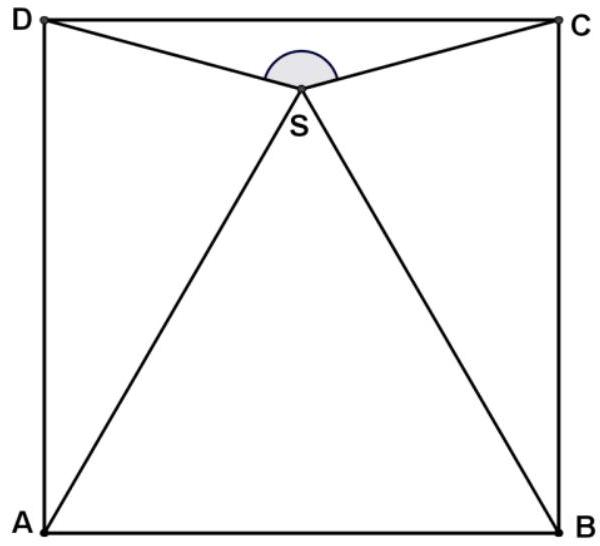
\includegraphics[max width=\textwidth, center]{2024_11_21_0810e0f7cfc837eac19bg-1}


\end{document}